\section{Beobachter}

Bisher wurde von einer wesentlichen Vereinfachung der Realität ausgegangen. Nämlich dass für Stabilisierung, Zustandsrückführung \etc der gesamte Zustandsvektor des Kontrollsystems zur Verfügung steht. Tatsächlich sind in der Regel nicht alle Zustandsinformationen bekannt. Beispielsweise weil sie technisch überhaupt nicht messbar sind oder nur unter großem technischen beziehungsweise finanziellen Aufwand ermittelt werden könnten. Sprachlich wird
vereinfacht gesagt, dass die entsprechenden Größen \textit{nicht messbar} sind.

\begin{align*}
    dim(y) < dim(x)
\end{align*}

\begin{figure}[H]
    \centering
    \fbox{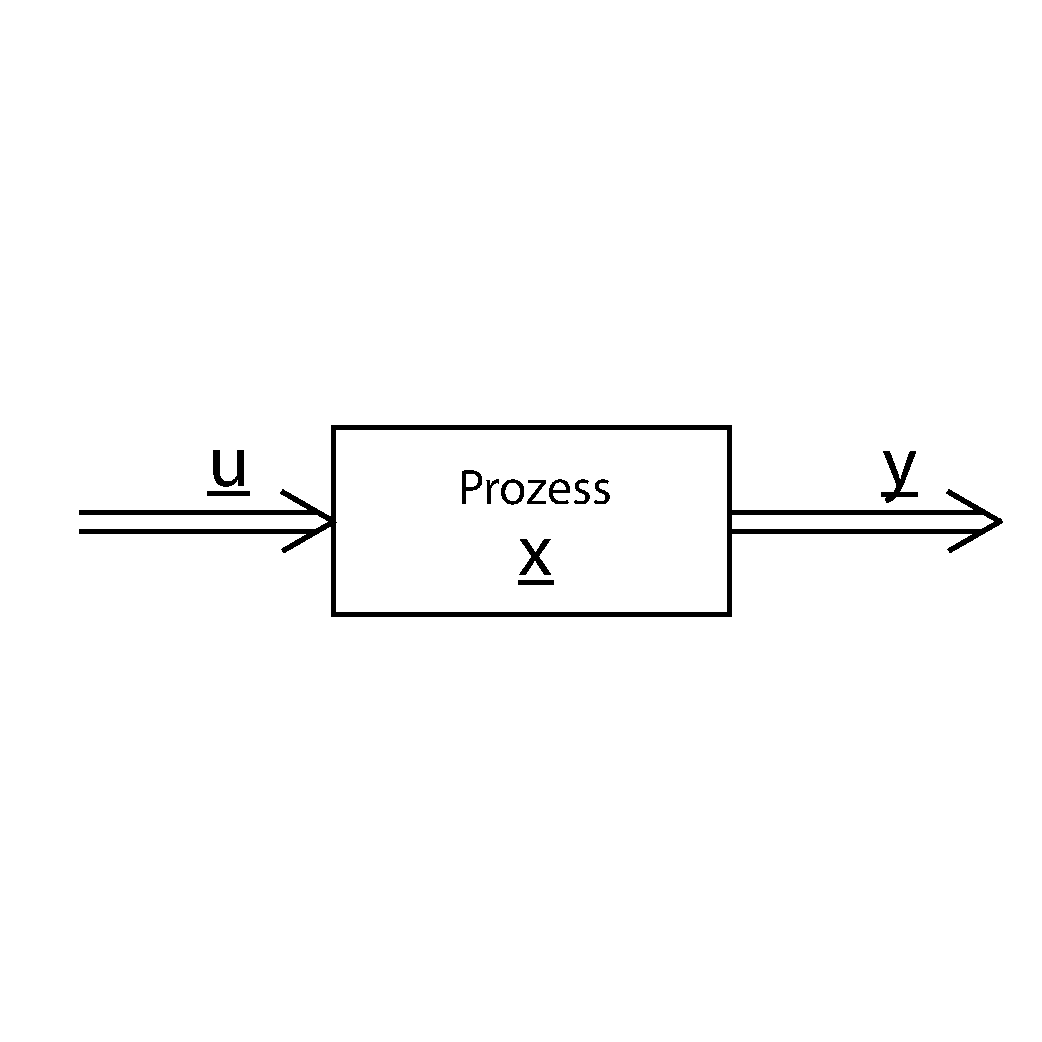
\includegraphics[width=0.5\textwidth]{Bilder/Beobachter/System.pdf}}
    \caption[Allgemeines System im Zustandsraum]{Schematische Darstellung eines allgemeinen Systems im Zustandsraum}
    \label{fig:Bild43}
\end{figure}

Da aber dennoch alle Zustände benötigt werden, da die Zustandsregelung darauf basiert, dass zu jedem Zeitpunkt alle Zustände bekannt sind, wird der Beobachter eingeführt.\\
Mit dessen Hilfe ist es möglich innere Zustände zu rekonstruieren. Dies erfolgt über ein \textbf{Modell} und dem \textbf{Vergleich} der rekonstruierten Zustände mit den gemessenen Ausgängen.\\
\newline
Ansatz von Luenberger:

\[
    \underline{\dot{\hat{x}}} = 
    \underbrace{% 
        A \cdot \underline{\hat{x}} + B \cdot \underline{u}
    }_{%
    Modell
    }
    + 
    \underbrace{%
    L \left( \underline{y} - \underline{\hat{y}}\right)
    }_{%
    Vergleich
    }
\]
\[
    \underline{\hat{y}} = C \cdot \underline{\hat{x}}
\]

Im Fall des behandelten inversen Pendels kann die Winkelgeschwindigkeit $\dot{\varphi}$ nicht gemessen werden, sondern muss über den Beobachter rekonstruiert werden. Der mathematische Ansatz und die Umsetzung in Matlab/Simulink sind in den beiden folgenden Unterabschnitten beschrieben.

\begin{figure}[H]
    \centering
    \fbox{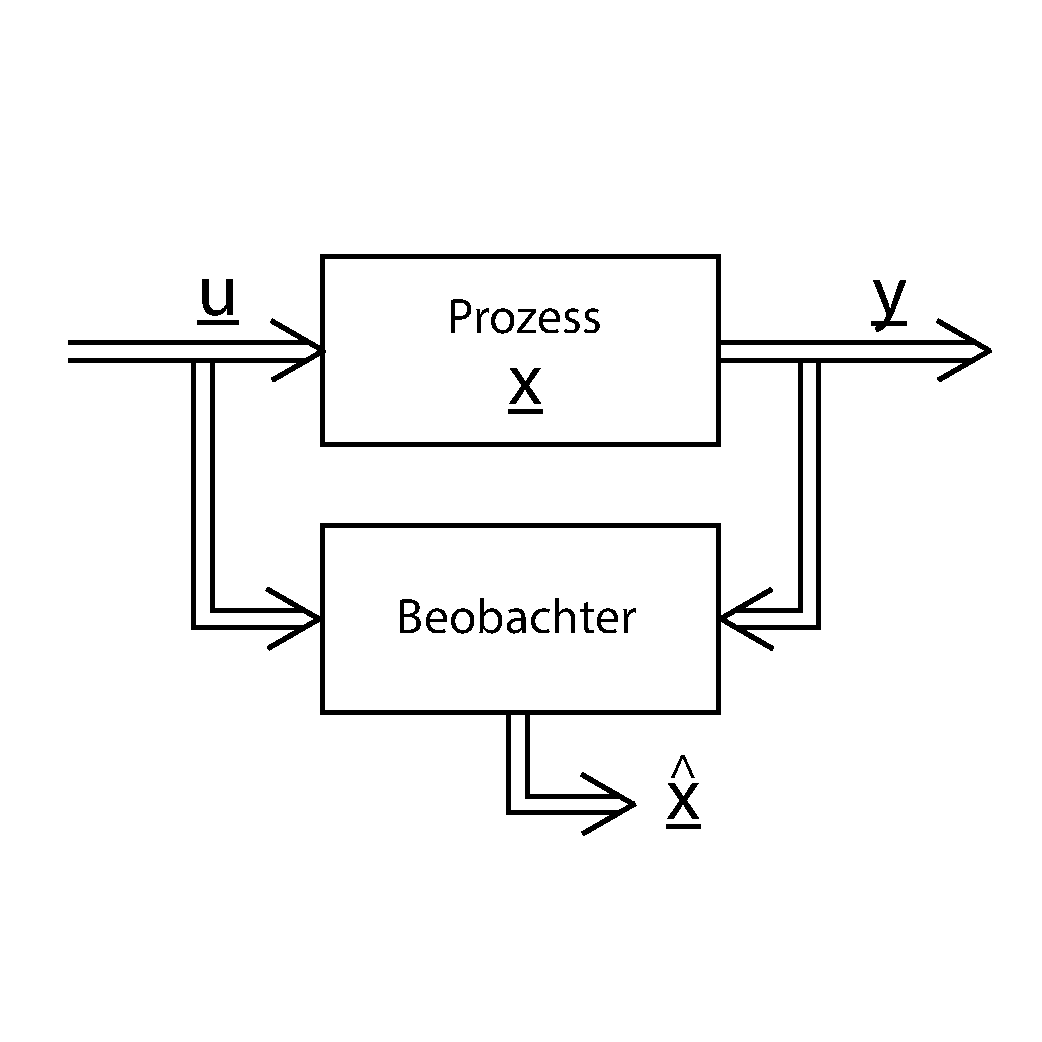
\includegraphics[width=0.5\textwidth]{Bilder/Beobachter/System_Beobachter.pdf}}
    \caption[System mit Beobachter]{Schematische Darstellung eines allgemeinen Systems mit Beobachter im Zustandsraum}
    \label{fig:Bild44}
\end{figure}

\subsection{Überprüfung der Beobachtbarkeit}

Naheliegend ist zunächst die Überlegung anzustellen, wann sich der Gesamtzustand $\underline{x}$ aus dem Ausgang $\underline{y}$ rekonstruieren lässt. Dies wird auch \textbf{Beobachtbarkeit} des Systems genannt. Konkret gilt der Satz: \\
\newline
\textit{Ein System ist beobachtbar, falls mit der Messung von $\underline{u}$ und $\underline{y}$ nach endlicher Zeit $t$ der unbekannte Zustandsvektor $\underline{x}$ vom System rekonstruiert werden kann.} \\
\newline
Der Beobachter lässt sich auf die Klasse der linearen zeitinvarianten Systeme (LTI) anwenden:

\begin{align}
    \underline{\dot{\hat{x}}} = A \cdot \underline{\hat{x}} + B \cdot \underline{u} + L \left( \underline{y} - C \cdot \underline{\hat{x}}\right)
\end{align}

Ein System ist vollständig beobachtbar, falls für die Beobachtbarkeitsmatrix

\begin{align}
    Q_{\mathrm{Obs}} =
    \begin{pmatrix}
        C \\
        C \cdot A \\
        \vdots \\
        C \cdot A^{n - 1}
    \end{pmatrix}
\end{align}

mit $n\in\mathbb{N}$, $p\in\mathbb{N}$, $A\in\mathbb{R}^{(n\times n)}$, $C\in\mathbb{R}^{(p\times n)}$ für SISO Systeme

\begin{align}
    det(Q_{\mathrm{Obs}}) \neq 0
\end{align}

und für MIMO \bzw SIMO Systeme

\begin{align}
    rank(Q_{\mathrm{Obs}}) = n \quad \text{\bzw} \quad m
\end{align}

gilt, wobei $n$ die Anzahl der linear unabhängigen Zeilen einer Matrix ist und $m$ die Anzahl der linear unabhängigen Spalten. Falls

\begin{align*}
    n &> m: \\
    rank(X) &= m
\end{align*}

und falls

\begin{align*}
    m &> n: \\
    rank(X) &= n.
\end{align*}

Die konkrete C-Matrix für das inverse Pendel

\begin{align}
    C_{\mathrm{Obs}} = 
    \begin{bmatrix}
        1 & 0 & 0 & 0 \\
        0 & 0 & 1 & 0 \\
        0 & 0 & 0 & 1
    \end{bmatrix}
\end{align}

besitzt p Zeilen, wobei sich die Anzahl der Zeilen nach den messbaren Zuständen richtet. Zu erkennen ist, dass bei der Betrachtung nicht wie beim Zustandsreglerentwurf ein SISO System angenommen werden kann, sondern ein SIMO System auf Beobachtbarkeit untersucht wird. Somit muss der Rang der Beobachtbarkeitsmatrix bestimmt werden.\\
Das Aufstellen der Beobachtbarkeitsmatrix führt zu

\begin{align}
    Q_{\mathrm{Obs}} = 
    \begin{bmatrix}
        1 & 0 & 0 & 0 \\
        0 & 0 & 1 & 0 \\
        0 & 0 & 0 & 1 \\
        0 & 1 & 0 & 0 \\
        0 & 0 & 0 & 1 \\
        -0.8502 & 0.0008 & 0 & -2.3333 \\
       26.6505 & -0.0248 & 0 & 5.8333 \\
       -0.8502 & 0.0008 & 0 & -2.3333 \\
        2.0049 & -0.8521 & 0 & 5.4491 \\
       -5.6209 & 26.6557 & 0 & -13.7559 \\
        2.0049 & -0.8521 & 0 & 5.4491 \\
      -27.3408 & 2.0304 & 0 & -17.6849
    \end{bmatrix}.
\end{align}

Der Rang folgt zu:

\begin{align}
    rank(Q_{\mathrm{Obs}}) = 4
\end{align}

Da $m > n$ muss $n = 4$ gelten. Da dies der Fall ist, ist das System beobachtbar.

\subsection{Beobachterentwurf}

Wie bereits bei der Untersuchung der Beobachtbarkeit festgestellt wurde, handelt es sich bei dem zu beobachtenden System um ein SIMO System. Im Folgenden soll der Beobachter auf einen Zustandsregler mit I-Regelung (wie bereits in \autoref{sec:iregler} mit Referenzwertvorgabe für $x_{\mathrm{M}}$) angewendet werden. Damit der Beobachter auf diesen Regler angewendet werden kann, muss dieser zunächst implementiert werden. Im Gegensatz zu \autoref{sec:iregler} wird wie bereits festgestellt ein SIMO-System geregelt. Dazu müssen bevor der Beobachterentwurf stattfinden kann zunächst passende k-Faktoren über die Formulierung von linearen Matrixungleichungen gefunden werden, um den Regler umzusetzen. Als Ansatz gelten die \textbf{Quadratischen Ljapunov Funktionen}:

\begin{align}
    V = \underline{x}^T \cdot P \cdot \underline{x} \quad mit \quad P > 0 \quad , \quad P = P^T
\end{align}

Gewählt wurde weiterhin der Ansatz für exponentielle Stabilität. Gesucht ist somit

\begin{align}
    \dot{V} < -2\alpha \cdot V
\end{align}

mit $\alpha > 0$ als als vorgegebene Abklingrate (Decay-Rate).\\
\newline
Mit dem Kriterium für exponentielle Stabilität folgt:

\[
    \underbrace{% 
        \underline{x}^T \cdot \left( a^TP + PA\right) \cdot \underline{x}
    }_{%
    \dot{V}
    }
    < 
    \underbrace{%
    -2\alpha \cdot \underline{x}^TP\underline{x}
    }_{%
    -2\alpha V
    }
\]

\begin{align}
    \underline{x}^T \cdot \left( A^TP + PA + 2\alpha P\right) \cdot \underline{x} < 0
\end{align}

Dies ist erfüllt, falls die zusammengesetzte Matrix negativ definit ist, also 

\begin{align}
    A^TP + PA + 2\alpha P < 0
\end{align}

gilt.\\
\newline
Zusammengefasst ergibt sich das \textit{Kriterium zur exponentiellen Stabilität} mit geforderter Abklingrate:

\begin{align} \label{eq:Gleichung82}
    \begin{split}
        A^T + PA + 2\alpha P < 0 \\
        P > 0
    \end{split}
\end{align}

Analog zu \autoref{sec:iregler} wird die Matrix C wie folgt gewählt:

\begin{align*}
    C = 
    \begin{bmatrix}
        0 & 0 & 1 & 0
    \end{bmatrix}
\end{align*}

Ebenfalls müssen wieder $\tilde{A}$ und $\tilde{B}$ bestimmt werden:

\begin{align*}
    \underline{\tilde{A}} &= 
    \begin{bmatrix}
        \underline{A} & \underline{0} \\
        -\underline{C} & \underline{0}
    \end{bmatrix} \quad ; \underline{\tilde{A}}\in\mathbb{R}^{(n+p)x(n+p)}\\
    \underline{\tilde{B}} &= 
    \begin{bmatrix}
        \underline{B} \\
        \underline{0}
    \end{bmatrix}\qquad ; \underline{\tilde{B}}\in\mathbb{R}^{(n+p)x(m)}
\end{align*}

Zuletzt wird $\alpha$ gewählt zu

\begin{align*}
    \alpha = 0.6.
\end{align*}

Über die LMI-Funktionen in Matlab kann nun die lineare Matrixungleichung in \autoref{eq:Gleichung82} gelöst werden.\\\\
Die $\underline{\tilde{k}}$-Matrix mit $K = MX^{-1}$ resultiert zu:

\begin{align}
    \underline{\tilde{k}} &= 
    \begin{bmatrix}
        -314.9301 & -58.3101 & -108.2878 & -84.0734 & 59.0425
    \end{bmatrix}
\end{align}

Gemäß \autoref{eq:Gleichung62} folgen die Verstärkungskoeffizienten wie nachfolgend gezeigt:\\\\
Zustandsrückführungskoeffizienten:

\begin{align}
    \underline{k}_{\mathrm{x}} &= 
    \begin{bmatrix}
        -314.9301 & -58.3101 & -108.2878 & -84.0734
    \end{bmatrix}
\end{align}

I-Verstärkungskoeffizienten:

\begin{align}
    \underline{k}_{\mathrm{I}} &= [-59.0425]
\end{align}

Die Polstellen des Reglers können abschließend berechnet werden über:

\begin{align}
    \begin{split}
        \underline{s}_{\mathrm{P}} &= eig(A - Bk) \\&=
        \begin{bmatrix}
            -9.4 + 5.1i & -9.4 - 5.1i & -1.2 + 0i & -1.5 + 1.2i & -1.5 - 1.2i
        \end{bmatrix}
    \end{split}
\end{align}

\begin{figure}[H]
    \centering
    \fbox{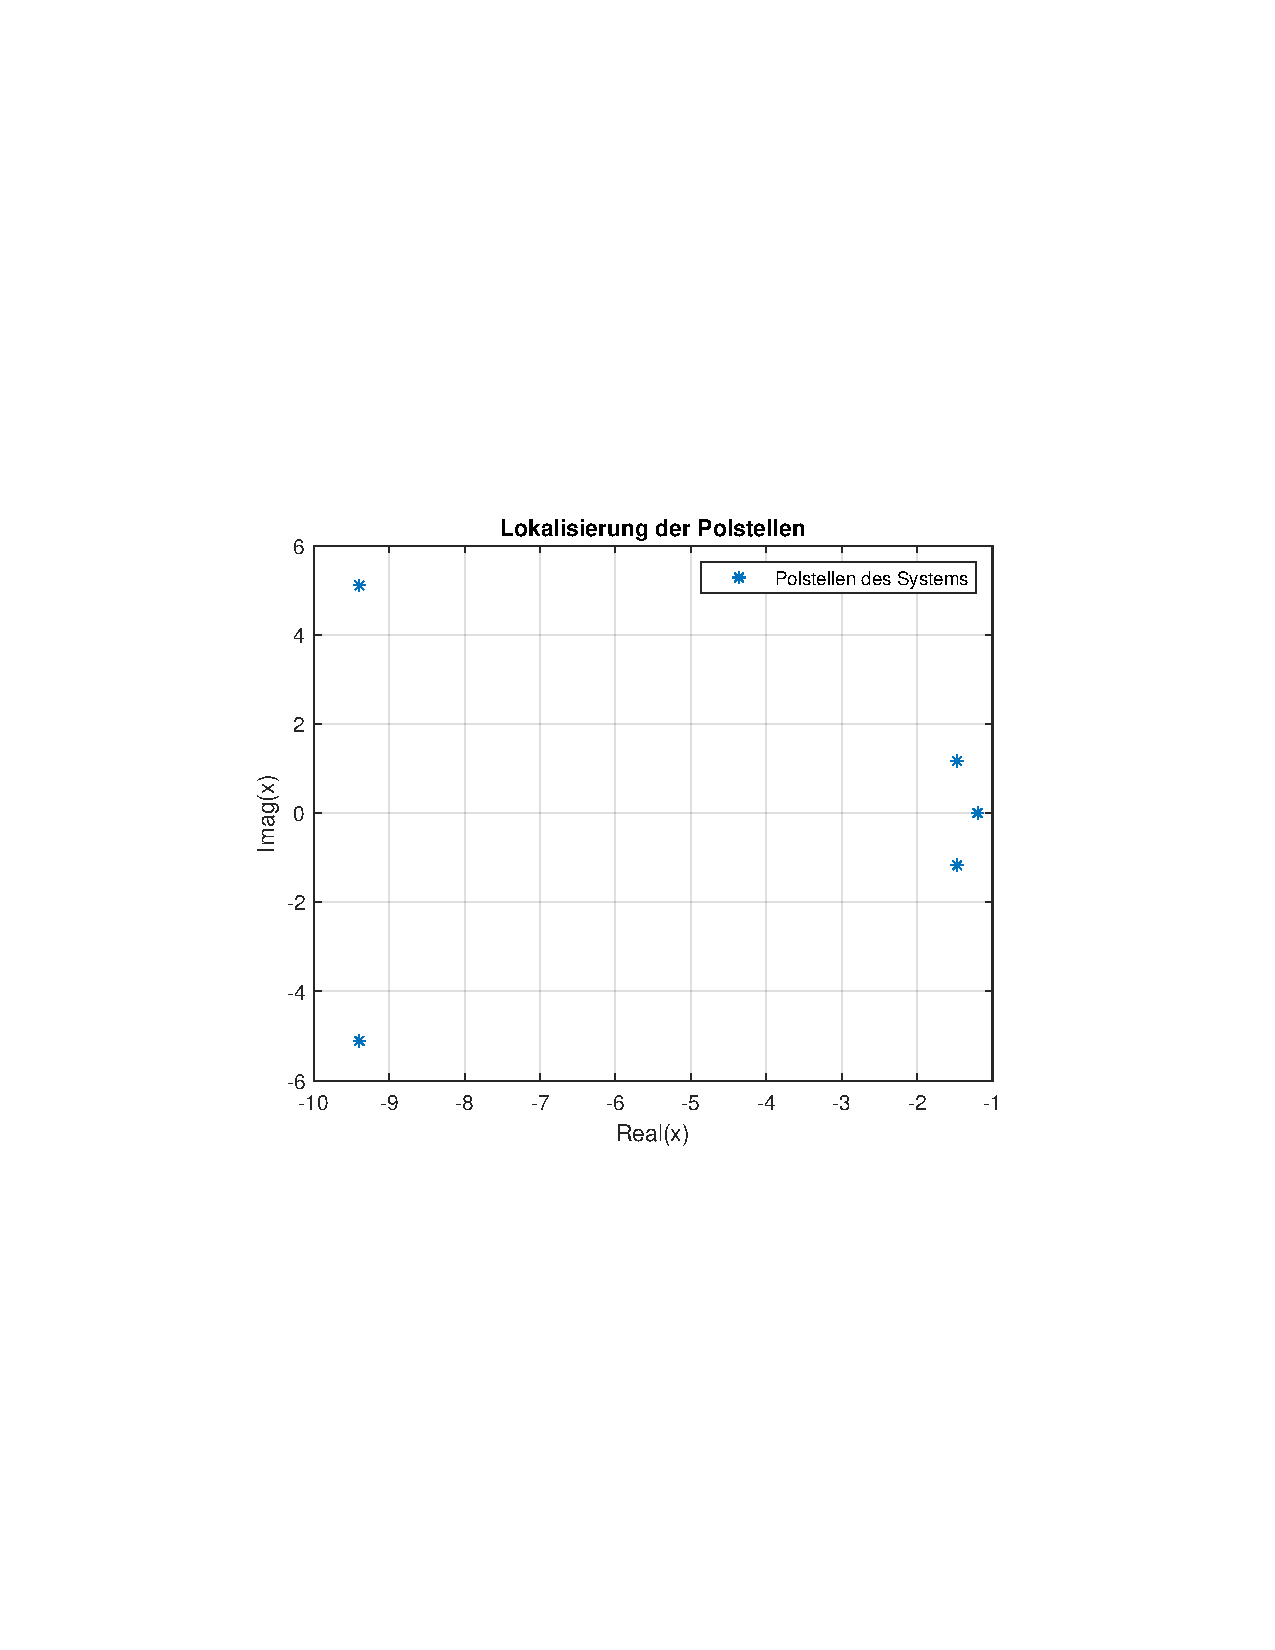
\includegraphics[width=0.75\textwidth]{Bilder/Polstellen_Regler_LMI.pdf}}
    \caption[Polstellen Regler mit LMI]{Polstellenlage des Systems mit I-Regelung und LMI}
    \label{fig:Bild45}
\end{figure}

Nachdem der Regler nun erfolgreich über LMI's implementiert wurde, kann nun mit dem Beobachterentwurf fortgesetzt werden.\\
Eine wichtige Erkenntnis wurde bis jetzt vorenthalten. zwischen dem Zustandsreglerentwurf und dem Beobachterentwurf besteht eine \textbf{Dualität}. Das heißt konkret, das erneut der Ansatz mit quadratischen Ljapunov-Funktionen angesetzt werden kann, um den Beobachter umzusetzen.

\begin{align}
    V(\underline{e}) = \underline{e}^T \cdot P \cdot \underline{e} \quad mit \quad V(\underline{e}) > 0 \quad , \quad \underline{e} \neq 0 
\end{align}

Auch hier wird ein Beobachter mit Abklingrate gewählt, um diesmal einen exponentiellen Verlauf des Beobachterfehlers zu ermöglichen. Über $\alpha$ kann die Abklingrate des Fehlers genau eingestellt werden. Gesucht ist nun:

\begin{align}
    \dot{V}(\underline{e}) + 2 \cdot \alpha \cdot V(\underline{e}) < 0
\end{align}

Somit kann analog zum Regler eine LMI Formulierung vorgenommen werden:

\begin{align} \label{eq:Gleichung89}
    \begin{split}
        A^T + PA - NC - C^TN + 2\alpha P < 0 \\
        P > 0
    \end{split}
\end{align}

Zuletzt wird $\alpha$ gewählt zu

\begin{align*}
    \alpha _{Obs} = 4.0.
\end{align*}

Über die LMI-Funktionen in Matlab kann nun die lineare Matrixungleichung in \autoref{eq:Gleichung89} gelöst werden.\\\\
Die L-Matrix mit $L = P^{-1}N$ resultiert zu:

\begin{align}
    L &= 
    \begin{bmatrix}
        9.7627 & -0.1421 & 1.1786 \\
        72.8250 & -0.6596 & 11.3192 \\
        0.2876 & 4.5000 & 1.0417 \\
        -3.2221 & -0.0416 & 2.1657
    \end{bmatrix}
\end{align}

Die Polstellen des Beobachters können abschließend berechnet werden über:

\begin{align}
    \begin{split}
        \underline{s}_{\mathrm{P}} &= eig(A - LC) \\&=
        \begin{bmatrix}
            -4.9 + 5.0i & -4.9 - 5.0i & -4.5 + 0.03i & -4.5 - 0.03i
        \end{bmatrix}
    \end{split}
\end{align}

\begin{figure}[H]
    \centering
    \fbox{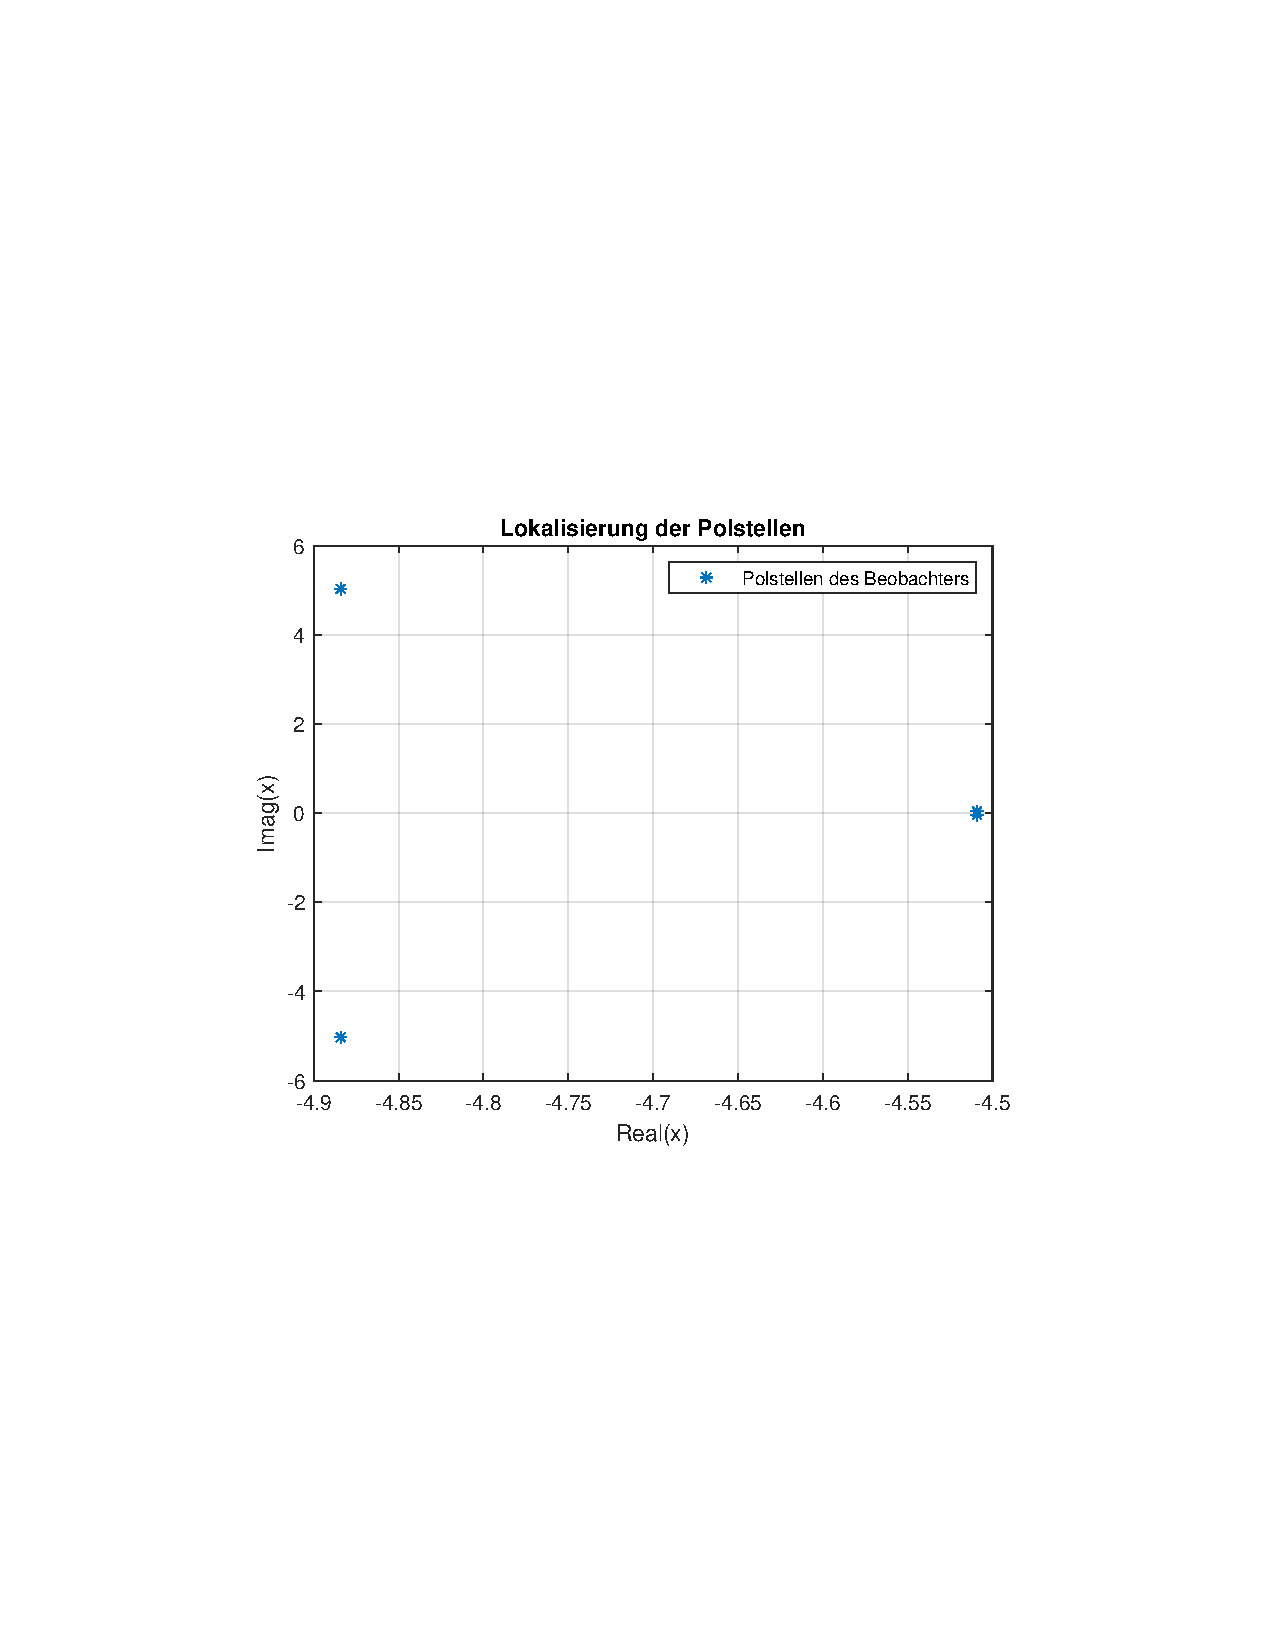
\includegraphics[width=0.75\textwidth]{Bilder/Polstellen_Beobachter_LMI.pdf}}
    \caption[Polstellen des Beobachters]{Polstellenlage des Beobachters}
    \label{fig:Bild46}
\end{figure}

Wichtig dabei ist zu beachten, dass die Polstellen des Beobachter schneller sein müssen, als die des geschlossenen Regelkreises (also links von diesen liegen müssen). Es gilt:

\begin{align}
    \left| Re\{ \underline{s}_{\mathrm{P}_{Obs}}\}\right| > \left| Re\{ \underline{s}_{\mathrm{P}_{Regler}}\}\right| \cdot (2 ... 3)
\end{align}

\autoref{fig:Bild47} zeigt die Systemstruktur des Zustandsreglers mit I-Regelung inklusive Beobachter.

\begin{figure}[H]
    \centering
    \fbox{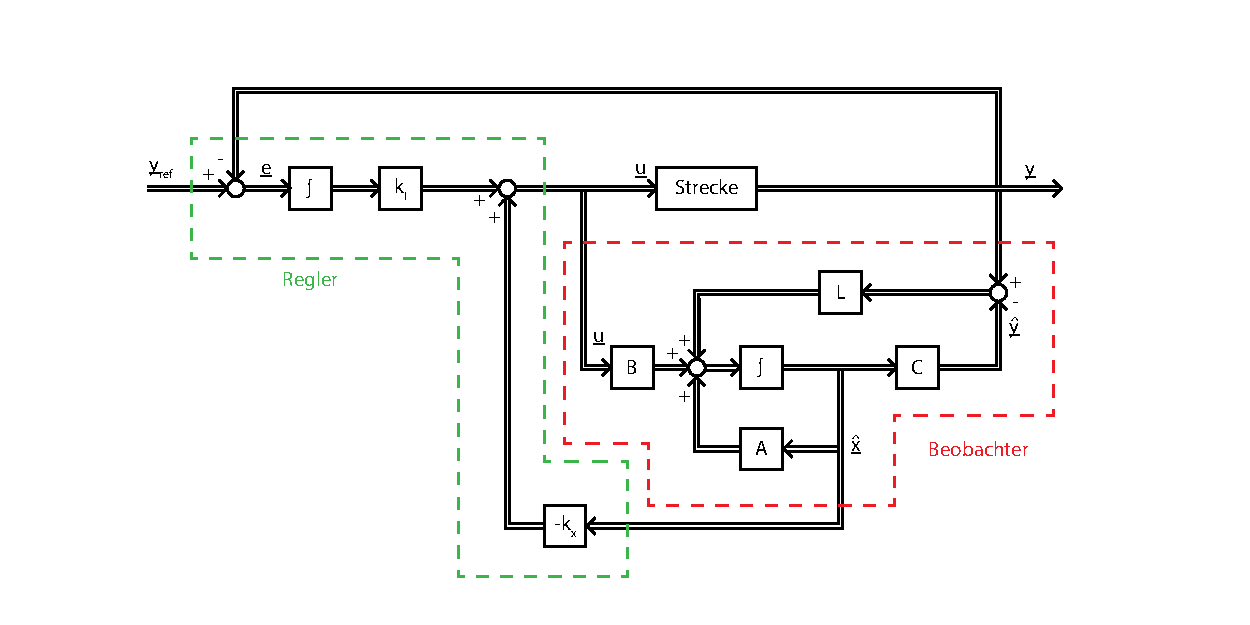
\includegraphics[width=1.0\textwidth]{Bilder/Beobachter/Beobachter_Regler_Strecke.pdf}}
    \caption[Reglerstruktur mit Beobachter]{Schematische Darstellung des Zustandsreglers mit I-Regelung und Beobachter}
    \label{fig:Bild47}
\end{figure}

\subsection{Beobachtervalidierung}

Im letzten Unterabschnitt der Arbeit soll der entwickelte Beobachter auf seine Funktionstüchtigkeit validiert werden. Wie bereits im vorangegangenen Abschnitt postuliert, wird der Beobachter auf den Zustandsregler mit I-Regelung angewendet. Das Modell in Simulink wird entsprechend des entworfenen Schemas in \autoref{fig:Bild47} umgesetzt. \autoref{fig:Bild48} zeigt die Blockstruktur des Beobachters, welcher mit in den Regelkreis integriert wurde. $\underline{\hat{x}}$ enthält die vier rekonstruierten Zustände des Systems. Unter anderem ist dort auch der Zustand $\dot{\varphi}$ wiederzufinden, der wie eingangs erwähnt nicht gemessen, sondern ausschließlich über den Beobachter ermittelt werden kann. \autoref{fig:Bild49} zeigt das Ergebnis der erfolgreichen Rekonstruktion der Winkelgeschwindigkeit des Pendels. Der Kurvenverlauf verhält sich ähnlich zum Messbaren Winkel $\varphi$ des Systems. Weiterhin ist zu erkennen, dass die Winkelgeschwindigkeit wieder zu $0 m/s$ ausgeregelt wird, was ebenfalls plausibel ist, da das Pendel wieder in der Ruhelage verharrt, sobald eine Eingangsstörung (in diesem Fall eine Auslenkung von $20^\circ$) auf das System eingeprägt wird.

\begin{figure}[H]
    \centering
    \fbox{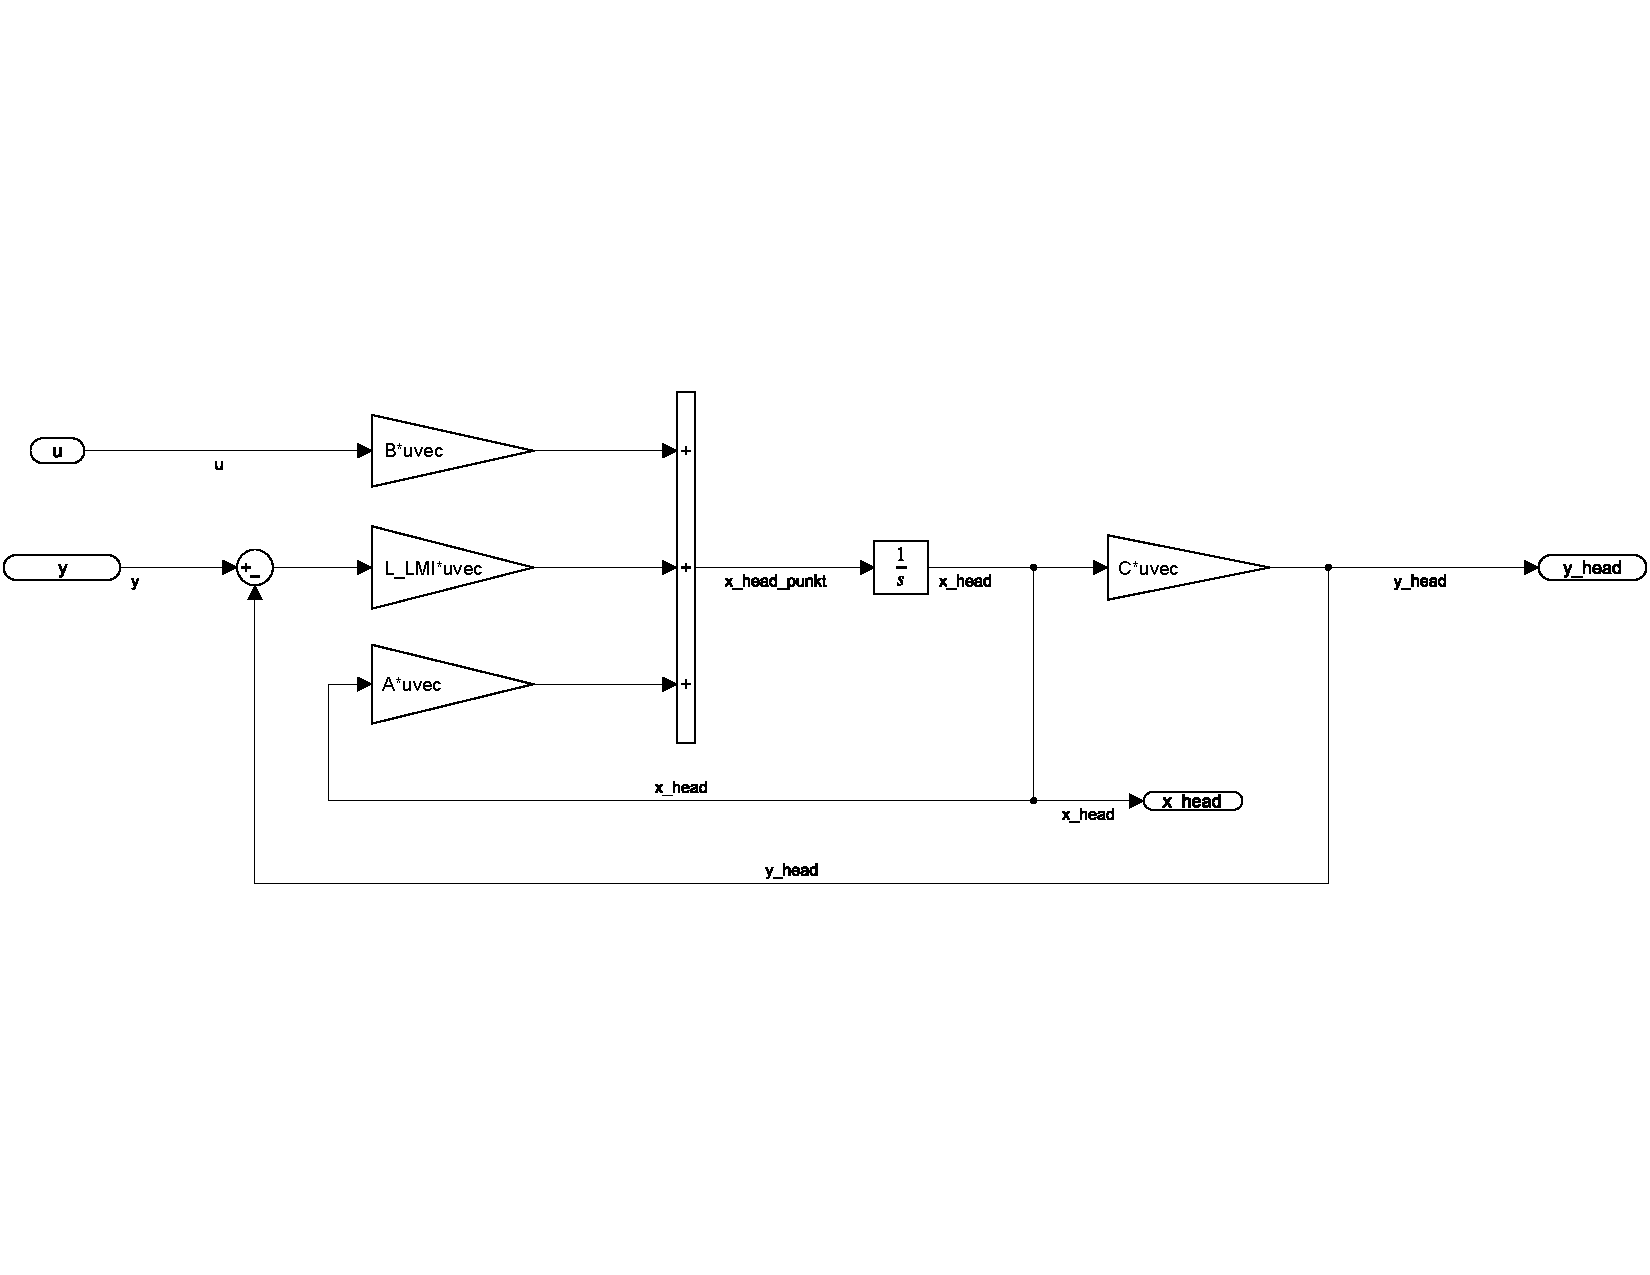
\includegraphics[width=1.0\textwidth]{Bilder/Beobachter/Simulink_Beobachter.pdf}}
    \caption[Beobachter Simulink]{Simulink Beobachter-Blockschaltbild für Zustandsregler mit I-Regelung und LMI}
    \label{fig:Bild48}
\end{figure}

\begin{figure}[H]
    \centering
    \fbox{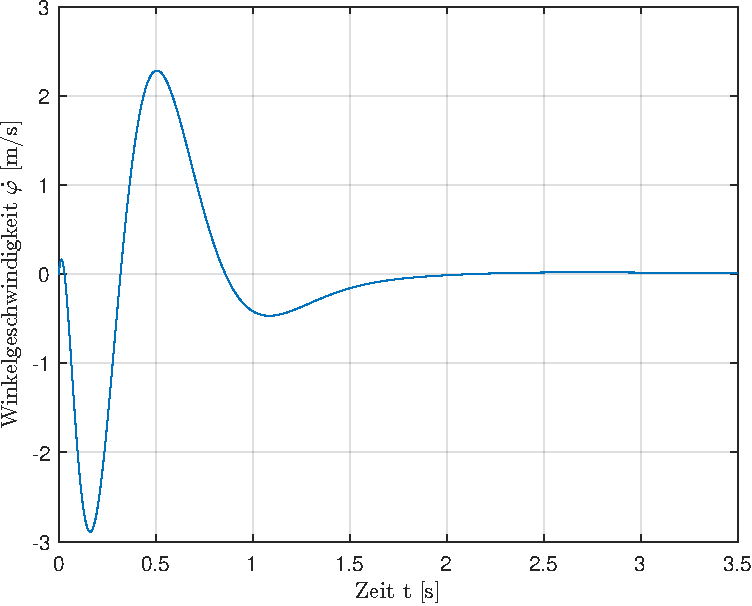
\includegraphics[width=0.6\textwidth]{Bilder/Beobachter/rekonstruktion_phi_punkt.pdf}}
    \caption[Rekonstruktion $\dot{\varphi}$]{Ergebnis der Rekonstruktion von $\dot{\varphi}$ über den Beobachter}
    \label{fig:Bild49}
\end{figure}

Anschließend werden die messbaren Zustände $\varphi$, $x_M$ und $\dot{x}_M$ mit den zugehörigen rekonstruierten Zuständen $\hat{\varphi}$, $\hat{x}_M$ und $\hat{\dot{x}}_M$ verglichen, um zu Prüfen, wie groß die durch den Beobachter erzeugten Abweichungen zwischen den realen und den rekonstruierten Zuständen sind. In \autoref{fig:Bild50} fällt auf, dass die Abweichungen zu beginn vergleichsweise groß sind, jedoch über wenige Sekunden annähernd verschwinden. Grund für die anfängliche Differenz zwischen $\varphi$ und $\hat{\varphi}$ ist das Integrationsglied im Beobachter, welches bei Null startet. Da der Winkel $\varphi$ auf Grund der eingeprägten Anfangsauslenkung nicht bei $0^\circ$ startet sondern bei $20^\circ$, die Integration jedoch bei Null beginnt, weist der dargestellte Kurvenverlauf eine anfängliche Abweichung von $20^\circ$ auf. Diese ist jedoch nach \ca einer Sekunde schon ausgeglichen. 

\begin{figure}[H]
    \centering
    \fbox{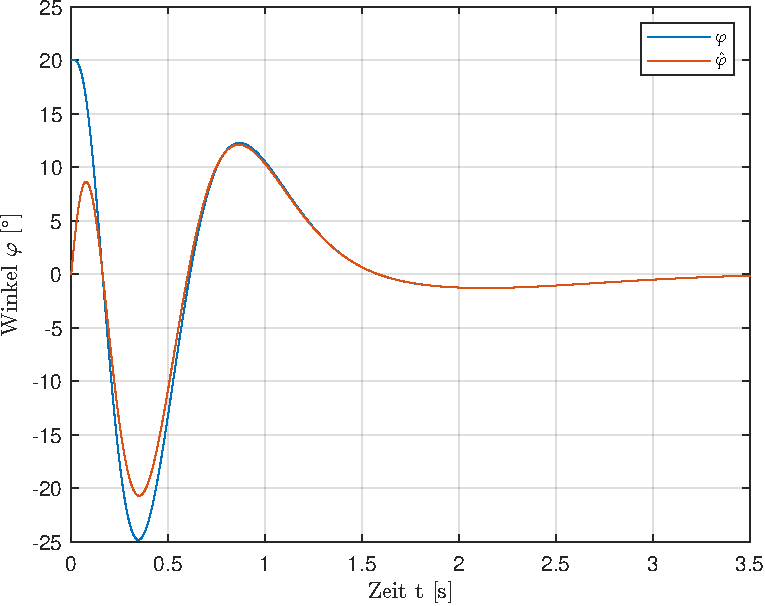
\includegraphics[width=0.75\textwidth]{Bilder/Beobachter/vergleich_phi_phi_head.pdf}}
    \caption[Vergleich $\varphi$, $\hat{\varphi}$]{Validierung des Beobachters anhand von $\varphi$ über den Vergleich mit $\hat{\varphi}$ bei einer Anfangsauslenkungen von $20^\circ$ und einer Referenzposition $y_{ref} = 0,1 m$ am linearen Zustandsraummodell}
    \label{fig:Bild50}
\end{figure}

Bei der Position $x_M$ und der Geschwindigkeit $\dot{x}_M$ des Wagens (zu sehen in \autoref{fig:Bild51} und \autoref{fig:Bild52}) fallen keine signifikanten Unterschiede zwischen den Kurvenverläufen der rekonstruierten Zustände und der realen \bzw gemessenen Zustände auf. Somit kann geschlussfolgert werden, dass die Implementierung des Beobachters erfolgreich ist.

\begin{figure}[H]
    \centering
    \fbox{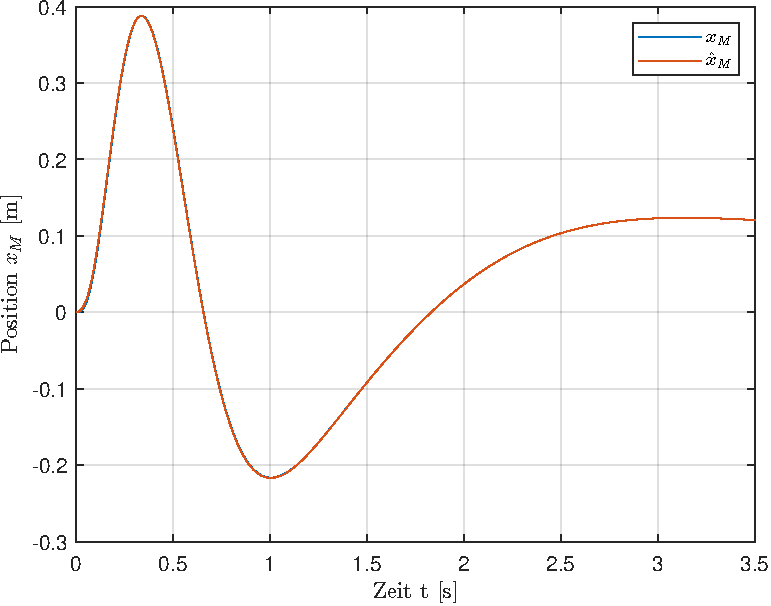
\includegraphics[width=0.6\textwidth]{Bilder/Beobachter/vergleich_xM_xM_head.pdf}}
    \caption[Vergleich $x_M$, $\hat{x}_M$]{Validierung des Beobachters anhand von $x_M$ über den Vergleich mit $\hat{x}_M$ bei einer Anfangsauslenkungen von $20^\circ$ und einer Referenzposition $y_{ref} = 0,1 m$ am linearen Zustandsraummodell}
    \label{fig:Bild51}
\end{figure}

\begin{figure}[H]
    \centering
    \fbox{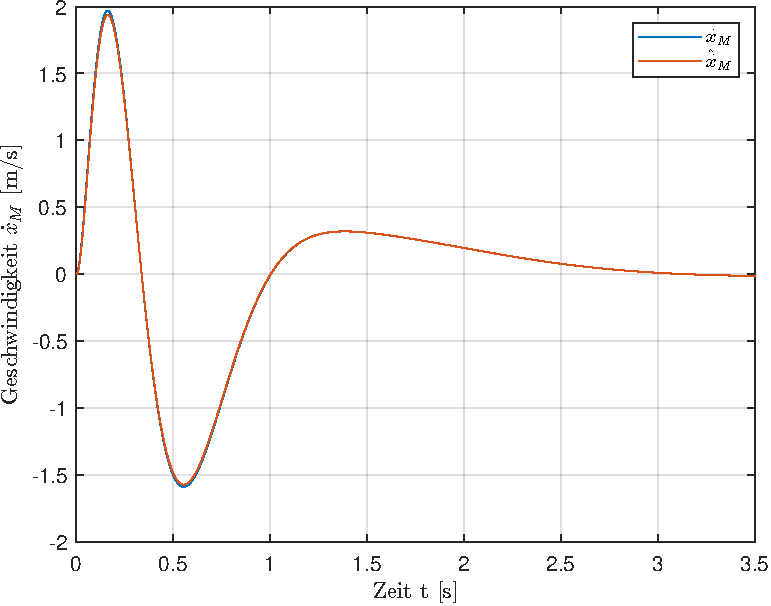
\includegraphics[width=0.6\textwidth]{Bilder/Beobachter/vergleich_xM_punkt_xM_punkt_head.pdf}}
    \caption[Vergleich $\dot{x}_M$, $\hat{\dot{x}}_M$]{Validierung des Beobachters anhand von $\dot{x}_M$ über den Vergleich mit $\hat{\dot{x}}_M$ bei einer Anfangsauslenkungen von $20^\circ$ und einer Referenzposition $y_{ref} = 0,1 m$ am linearen Zustandsraummodell}
    \label{fig:Bild52}
\end{figure}

Abschließend soll geprüft werden, ob die Systemgrenzen des Inversen Pendelversuchs für den umgesetzten Regler mit quadratischen Ljapunov-Funktionen und LMI's inklusive des Beobachters eingehalten werden. Wie auch schon bei der Reglervalidierung in \autoref{sec:reglervalidierung} werden zum einen die Eingangsparameter (Anfangsauslenkung und Referenzposition) variiert und zum anderen wird der Regler am linearen Modell getestet. Es wird dabei ausschließlich der im vorherigen Unterabschnitt entwickelte I-Regler untersucht. Auf die anderen Regelverfahren wurde verzichtet, da diese weniger effizient sind bei ähnlichem Ergebnis. Außerdem findet die Validierung ausschließlich an der linearen Regelstrecke statt, da die Ergebnisse des nicht-linearen Systems annähernd identisch sind, wie bereits in \autoref{sec:systemvergleich} nachgewiesen wurde. Zu prüfen ist, ob für die gewählten Abklingraten (Decay-Rate) des Reglers und des Beobachters sowohl die Grenzen der maximalen Wagenposition eingehalten werden ($ x_{M_{max}} = \pm 1 m$) als auch die maximale Eingangskraft des Motors ($u_{max} = 80 N$).\\
\newline
Zunächst wird der Winkel $\varphi$ des Pendels am Zustandsregler mit I-Regelung und Beobachter betrachtet. Die Ergebnisse der Simulation mit Simulink sind in \autoref{fig:Bild53} aufgezeigt. Der wesentliche Kurvenverlauf spricht mit dem I-Regler aus \autoref{fig:Bild22} überein. Unterschiede sind vor allem durch die Abweichenden Polstellen des Reglers zu begründen. Wurden zunächst in \autoref{sec:reglervalidierung} die Polstellen vorgegeben, so kamen nun durch den Ansatz mit quadratischen Ljapunov-Funktionen mit lediglich der Vorgabe einer Abklingrate andere Polstellen zustande. Weiterhin schwingt der Winkel im Vergleich zur Implementation ohne Beobachter etwas mehr über. Grund dafür ist die anfänglich größere Abweichung zwischen dem rekonstruierten Winkel des Pendels und dem Realen/Gemessenen. \\
\newline
Mit Hilfe von \autoref{fig:Bild54} kann erfolgreich nachgewiesen werden, dass die maximale Position des Wagens nicht überschritten wird. Weiterhin ist es möglich wie bei der I-Regelung in \autoref{sec:val_i_regler} eine Referenzposition vorzugeben, die nach dem Regelvorgang erreicht wird. Die Kurvenverläufe der Wagenposition mit Beobachter decken sich weitestgehend mit denen in \autoref{fig:Bild23}, wo noch kein Beobachter zur Zustandsrekonstruktion zum Einsatz kam. \\
\newline
\autoref{fig:Bild55} ist der Nachweis, dass für sämtliche Referenzpositionen innerhalb der Systemgrenzen bei einer maximalen Anfangsauslenkung von $24^\circ$ die Eingangskraft $u$ von maximal 80 N nicht überschritten wird. Bei einer Wahl der Abklingrate des Reglers von $\alpha_{Regler} = 0.6$ und einer Abklingrate des Beobachters mit $\alpha_{Obs} = 4$ wird die zur Verfügung stehende Eingangskraft maximal ausgereizt. Im Vergleich zu \autoref{fig:Bild24} (Eingangskraft bei I-Regler ohne Beobachter) fällt auf, dass erneut durch das Integrationsglied in der Beobachter Blockstruktur eine Anfängliche Abweichung auftritt.

\begin{figure}[H]
    \centering
    \fbox{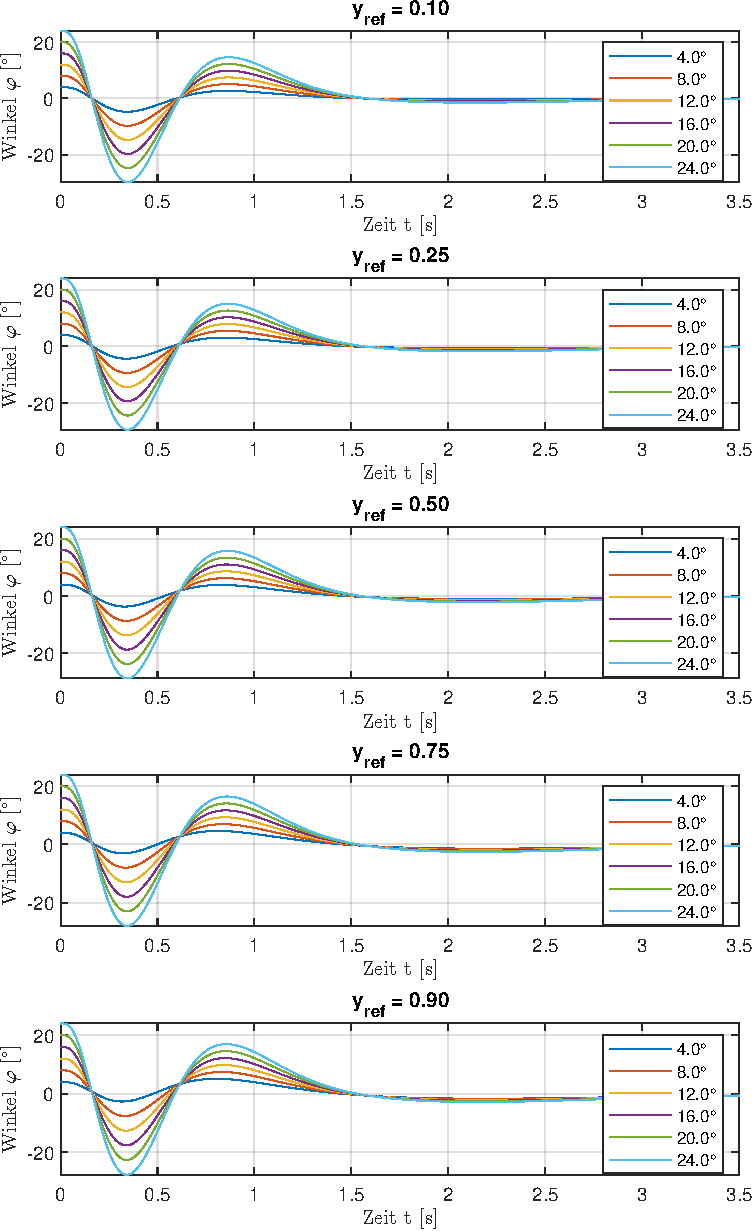
\includegraphics[width=0.76\textwidth]{Bilder/Beobachter/linear_lmi_i_regler_phi.pdf}}
    \caption[$\varphi$ für Regler mit I-Regelung und Beobachter (linear)]{$\varphi$ für verschiedene Referenzpositionen $y_{ref}$ und Anfangsauslenkungen am Zustandsregler mit I-Regelung und Beobachter für das lineare Zustandsraummodell}
    \label{fig:Bild53}
\end{figure}

\begin{figure}[H]
    \centering
    \fbox{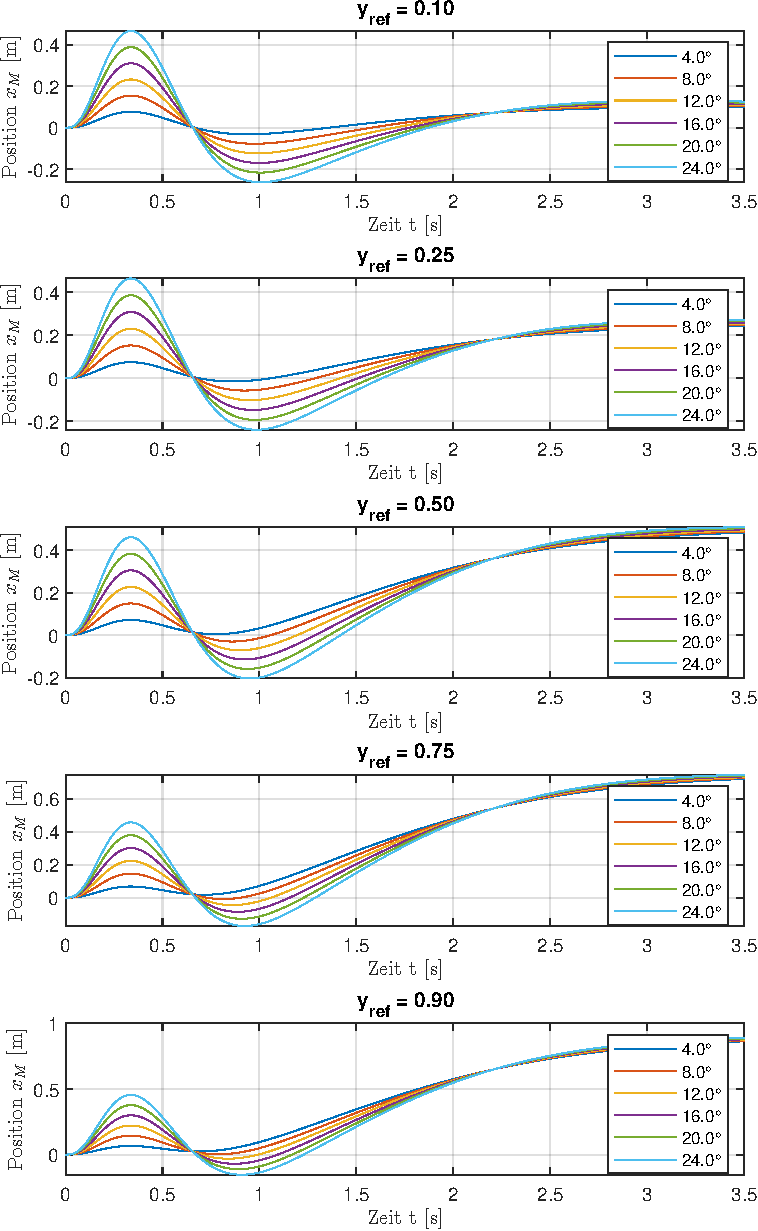
\includegraphics[width=0.76\textwidth]{Bilder/Beobachter/linear_lmi_i_regler_xM.pdf}}
    \caption[$x_M$ für Regler mit I-Regelung und Beobachter (linear)]{$x_M$ für verschiedene Referenzpositionen $y_{ref}$ und Anfangsauslenkungen am Zustandsregler mit I-Regelung und Beobachter für das lineare Zustandsraummodell}
    \label{fig:Bild54}
\end{figure}

\begin{figure}[H]
    \centering
    \fbox{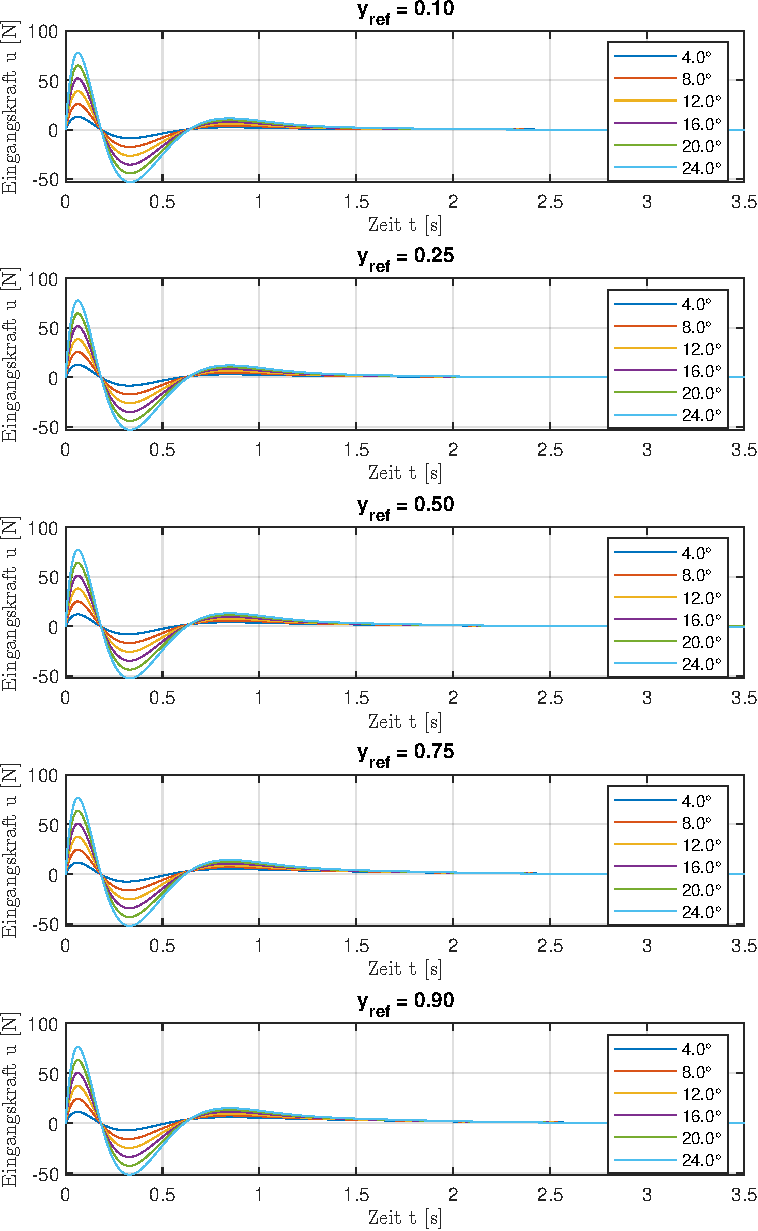
\includegraphics[width=0.76\textwidth]{Bilder/Beobachter/linear_lmi_i_regler_u.pdf}}
    \caption[$u$ für Regler mit I-Regelung und Beobachter (linear)]{$u$ für verschiedene Referenzpositionen $y_{ref}$ und Anfangsauslenkungen am Zustandsregler mit I-Regelung und Beobachter für das lineare Zustandsraummodell}
    \label{fig:Bild55}
\end{figure}